%%%%%%%%%%%%%%%%%%%%%%%%%%%%%%%%%%%%%%%%%%%%%%%%%%%%%%%%%%%%%%%%%%%%%%%%%%%%
% AGUJournalTemplate.tex: this template file is for articles formatted with LaTeX
%
% This file includes commands and instructions
% given in the order necessary to produce a final output that will
% satisfy AGU requirements, including customized APA reference formatting.
%
% You may copy this file and give it your
% article name, and enter your text.
%
% guidelines and troubleshooting are here: 

%% To submit your paper:
\documentclass[draft]{agujournal2019}
\usepackage{url} %this package should fix any errors with URLs in refs.
\usepackage{lineno}
\usepackage[inline]{trackchanges} %for better track changes. finalnew option will compile document with changes incorporated.
\usepackage{soul}
\linenumbers
%%%%%%%
% As of 2018 we recommend use of the TrackChanges package to mark revisions.
% The trackchanges package adds five new LaTeX commands:
%
%  \note[editor]{The note}
%  \annote[editor]{Text to annotate}{The note}
%  \add[editor]{Text to add}
%  \remove[editor]{Text to remove}
%  \change[editor]{Text to remove}{Text to add}
%
% complete documentation is here: http://trackchanges.sourceforge.net/
%%%%%%%

\draftfalse

%% Enter journal name below.
%% Choose from this list of Journals:
%
% JGR: Atmospheres
% JGR: Biogeosciences
% JGR: Earth Surface
% JGR: Oceans
% JGR: Planets
% JGR: Solid Earth
% JGR: Space Physics
% Global Biogeochemical Cycles
% Geophysical Research Letters
% Paleoceanography and Paleoclimatology
% Radio Science
% Reviews of Geophysics
% Tectonics
% Space Weather
% Water Resources Research
% Geochemistry, Geophysics, Geosystems
% Journal of Advances in Modeling Earth Systems (JAMES)
% Earth's Future
% Earth and Space Science
% Geohealth
%
% ie, \journalname{Water Resources Research}

%%%%%%%%%%%%%%%%%%%%%%%%%%%%%%%%%%%%%%%%%%%%%%%%%%%%%%%%%%%%%%%%%%%%%
%%%%%%%%%%%%%%%%%%%%%%%    REMOVE THIS    %%%%%%%%%%%%%%%%%%%%%%%%%%%
\hfuzz=10000pt
%%%%%%%%%%%%%%%%%%%%%%%%%%%%%%%%%%%%%%%%%%%%%%%%%%%%%%%%%%%%%%%%%%%%%
%%%%%%%%%%%%%%%%%%%%%%%%%%%%%%%%%%%%%%%%%%%%%%%%%%%%%%%%%%%%%%%%%%%%s

\journalname{Geophysical Research Letters}

\begin{document}

%%%%%%%%%%%%%%%%%%%%%%%%%%%%%%%%%%%%%%%%%%%%%%%
%  TITLE
%
% (A title should be specific, informative, and brief. Use
% abbreviations only if they are defined in the abstract. Titles that
% start with general keywords then specific terms are optimized in
% searches)
%
%%%%%%%%%%%%%%%%%%%%%%%%%%%%%%%%%%%%%%%%%%%%%%%

% Example: \title{This is a test title}

\title{Possible Causes of Increasing Aerosol Direct Effect Despite Declining Global Emissions in Recent Decades.}

%%%%%%%%%%%%%%%%%%%%%%%%%%%%%%%%%%%%%%%%%%%%%%%
%
%  AUTHORS AND AFFILIATIONS
%
%%%%%%%%%%%%%%%%%%%%%%%%%%%%%%%%%%%%%%%%%%%%%%%

% Authors are individuals who have significantly contributed to the
% research and preparation of the article. Group authors are allowed, if
% each author in the group is separately identified in an appendix.)

% List authors by first name or initial followed by last name and
% separated by commas. Use \affil{} to number affiliations, and
% \thanks{} for author notes.
% Additional author notes should be indicated with \thanks{} (for
% example, for current addresses).

% Example: \authors{A. B. Author\affil{1}\thanks{Current address, Antartica}, B. C. Author\affil{2,3}, and D. E.
% Author\affil{3,4}\thanks{Also funded by Monsanto.}}

\authors{Antoine Hermant\affil{1,2}, Linnea Huusko\affil{2}, Thorsten Mauritsen\affil{2}}

\affiliation{1}{Climate and Environmental Physics, Physics Institute, University of Bern, Bern, Switzerland}
\affiliation{2}{Department of Meteorology, Stockholm University, Stockholm, Sweden}

% \affiliation{=number=}{=Affiliation Address=}
%(repeat as many times as is necessary)


% Corresponding author mailing address and e-mail address:

% (include name and email addresses of the corresponding author.  More
% than one corresponding author is allowed in this LaTeX file and for
% publication; but only one corresponding author is allowed in our
% editorial system.)

% Example: \correspondingauthor{First and Last Name}{email@address.edu}

\correspondingauthor{Antoine Hermant}{antoine.hermant@misu.su.se}

%%%%%%%%%%%%%%%%%%%%%%%%%%%%%%%%%%%%%%%%%%%%%%%
% KEY POINTS
%%%%%%%%%%%%%%%%%%%%%%%%%%%%%%%%%%%%%%%%%%%%%%%
%  List up to three key points (at least one is required)
%  Key Points summarize the main points and conclusions of the article
%  Each must be 140 characters or fewer with no special characters or punctuation and must be complete sentences

% Example:
% \begin{keypoints}
% \item	List up to three key points (at least one is required)
% \item	Key Points summarize the main points and conclusions of the article
% \item	Each must be 140 characters or fewer with no special characters or punctuation and must be complete sentences
% \end{keypoints}

\begin{keypoints}
\item Despite declining aerosol emissions, the modelled direct effect of anthropogenic aerosols has continued to increase. 
\item Insights from the shift in aerosol pattern throughout the 1970--2014 period has implication in the continued increase in direct effect.
\item Regional variations in aerosol emission efficiency are associated with cloudiness, aerosol removal processes and surface albedo.
\end{keypoints}

%%%%%%%%%%%%%%%%%%%%%%%%%%%%%%%%%%%%%%%%%%%%%%%
%
%  ABSTRACT and PLAIN LANGUAGE SUMMARY
%
% A good Abstract will begin with a short description of the problem
% being addressed, briefly describe the new data or analyses, then
% briefly states the main conclusion(s) and how they are supported and
% uncertainties.

% The Plain Language Summary should be written for a broad audience,
% including journalists and the science-interested public, that will not have 
% a background in your field.
%
% A Plain Language Summary is required in GRL, JGR: Planets, JGR: Biogeosciences,
% JGR: Oceans, G-Cubed, Reviews of Geophysics, and JAMES.
% see http://sharingscience.agu.org/creating-plain-language-summary/)
%
%%%%%%%%%%%%%%%%%%%%%%%%%%%%%%%%%%%%%%%%%%%%%%%

%% \begin{abstract} starts the second page

\begin{abstract}
Anthropogenic aerosol particles partially mask global warming driven by greenhouse gases, both by directly reflecting sunlight back into space and indirectly by increasing cloud reflectivity, which also results in sunlight reflection. In recent decades, however, the emissions of anthropogenic aerosols have declined globally, and at the same time shifted from the North American and European regions to foremost Southeast Asia. Using simulations within the MPI-ESM1.2 global climate model with parametrised aerosols, we find that the direct effect of aerosols has instead continued to increase, despite declining emissions. Concurrently, the indirect effect has diminished in approximate proportion to emissions. The enhanced efficiency of aerosol emissions to the induced negative forcing is associated with less cloudiness, longer atmospheric residence time, and emissions over darker surfaces in the Southeast Asian region.
\end{abstract}

\section*{Plain Language Summary}
Aerosols, which are tiny particles in the atmosphere from natural sources and human activities, have a cooling effect on climate, partially masking global warming caused by greenhouse gases. They achieve this through both direct and indirect mechanisms. Directly, aerosols cool the climate by reflecting incoming sunlight, while indirectly, they alter cloud properties, increasing cloud reflectivity, further cooling the climate. In this study, we investigate the historical evolution of these effects using a global climate model. We discovered that despite their global decline, the direct effect of human-made aerosols on the climate has instead increased, while the indirect effect has decreased. We associate the increase in direct effect with the shift in aerosol spatial distribution that accompanied the decline. Our findings underscore the critical role of aerosol emission regions in climate impact, particularly evident for the indirect effect, which prevails in originally pristine areas. However, this regional dependence also applies to the direct effect, influenced by factors such as cloud cover, surface reflectivity (albedo), and the processes involved in aerosol removal from the atmosphere.

%Here are instructions on writing a Plain Language Summary: 
%https://www.agu.org/Share-and-Advocate/Share/Community/Plain-language-summary


%%%%%%%%%%%%%%%%%%%%%%%%%%%%%%%%%%%%%%%%%%%%%%%
%
%  BODY TEXT
%
%%%%%%%%%%%%%%%%%%%%%%%%%%%%%%%%%%%%%%%%%%%%%%%

%%% Suggested section heads:
% \section{Introduction}
%
% The main text should start with an introduction. Except for short
% manuscripts (such as comments and replies), the text should be divided
% into sections, each with its own heading.

% Headings should be sentence fragments and do not begin with a
% lowercase letter or number. Examples of good headings are:

% \section{Materials and Methods}
% Here is text on Materials and Methods.
%
% \subsection{A descriptive heading about methods}
% More about Methods.
%
% \section{Data} (Or section title might be a descriptive heading about data)
%
% \section{Results} (Or section title might be a descriptive heading about the
% results)
%
% \section{Conclusions}


\section{Introduction}
      %Global climate models participating in the Coupled Model Intercomparison Project phase 6 (CMIP6) have indicated a higher climate sensitivity comparing to previous models \cite{Flynn_2020}. However, a majority of these models simulate a reduced historical warming, with global temperatures consistently cooler than actual observations from 1940 to 2000. \citeA{Flynn_2023} has demonstrated that strong aerosol cooling alone cannot account for this lack of warming in the mid-20th century. 

      The state a the climate is determined by the balance between the incoming solar energy the Earth receives and the energy the Earth radiates back into space. Greenhouse gases, such as CO$_2$, act as positive forcings in this equilibrium by absorbing radiation emitted by the Earth's surface, resulting in an increase in surface temperature $T_s$. A linear radiative balance framework can be used to study the response in temperature $\Delta T_s$ to an applied forcing $F$ on the radiative balance at the top of the atmosphere $\Delta R$:
      \begin{equation}\label{eq:eq1}
            \Delta R = F + \lambda \Delta T_s,
      \end{equation}
      where $\lambda$ is the total feedback parameter of the system and must be negative to yield a stable climate. The feedback parameter can be itself divided into the sum of the individual climate feedbacks, such as water vapour, surface albedo, cloud and temperature feedbacks. They contribute to enhance or dampen the imbalance induced by an applied forcing.

      Aerosols are tiny particles emitted by natural and human sources, which disrupt the radiative balance of the climate system through direct and indirect effects. Directly, they interact with solar radiation by scattering and reflecting it back to space or absorbing it. Indirectly, they interact with clouds, for example through the Twomey effect \cite{Twomey_1974} by increasing the number density of droplets in clouds, making them more reflective to solar radiation. Due to their short lifetime in the atmosphere, aerosols are heterogeneously distributed, spatial and temporally, resulting in local effects on the radiation balance.
      Aerosols, especially their interactions with clouds, are the primary source of uncertainty when it comes to the overall radiative imbalance \cite{Forster_2021}. This uncertainty poses challenges in assessing how aerosols may mask the effects of global warming caused by greenhouse gases. Here, we seek to accurately dissociate the forcing induced by aerosols and their associated effects to other forcing agents and feedbacks in a climate model, which can help to better understand their past and present implications on climate change.

      The models participating in the Coupled Model Intercomparison Project (CMIP) exhibit a wide range of aerosol radiative forcing \cite{Bellouin_2020}. This range are primarily explained by differences in the magnitude of cloud-mediated effects \cite{Fiedler_2023}. Furthermore, these cloud-mediated effects induce stronger response due to cooling in remote regions compared to aerosol-radiation interactions that are more localised at emission sources \cite{Huusko_2022}. This highlights the importance of aerosol distribution in shaping the resulting forcing and cooling effect. However, the historical evolution of the relative contribution of the direct and indirect effects remains uncertain, as aerosol spatial distribution has changed with evolving emission patterns \cite{Stevens_2015}. Indeed, aerosol emission pattern has significantly changed over the past decades, reducing globally and shifting from North American and European regions to Southeast Asia.

      In this study, we propose employing the Partial Radiative Perturbation (PRP) method \cite{Wetherald_1988,Colman_1997,Klocke_2013} for calculating the aerosol instantaneous radiative forcing. We use this method alongside the simplified representation of anthropogenic aerosols from MACv2-SP \cite{Stevens_2017} in MPI-ESM1.2 \cite{Mauritsen_2019}, enabling the separation of direct (aerosol-radiation interactions) and indirect (aerosol-clouds interactions) effects. By using this approach, we can investigate the historical trends of both aerosol effects and gain insights into the mechanisms underlying the influence of aerosol spatial distribution on the resulting radiative forcing.

\section{Method}\label{sec:method}
      We study the historical evolution of the aerosol forcing using the Max Planck Institute for Meteorology Earth System Model version 1.2. MPI-ESM1.2, a state-of-the-art climate model \cite{Mauritsen_2019} that participated in the Coupled Model Intercomparison Project Phase 6 (CMIP6), successfully reproduces the observed warming from pre-industrial levels \cite{Mauritsen_2020}.
      The radiative transfer scheme of MPI-ESM1.2 uses the Simple Plumes implementation of the second version of the Max Planck Institute Aerosol Climatology (MACv2-SP) to represent the aerosol impact on the radiation. 
      
      MACv2-SP provides a parametrization of optical properties of anthropogenic aerosols and the resulting Twomey effect \cite{Twomey_1974}, accounting for aerosol-cloud interaction \cite{Stevens_2017}. It has been designed with the desire of an uniform and easily controlled representation of anthropogenic aerosol perturbations for the CMIP6 framework \cite{Eyring_2016,Pincus_2016}. To achieve this, \citeA{Stevens_2017} constructed nine spatial plumes that are associated with emissions from major anthropogenic source regions. They used aerosol optical properties estimates from ground-based measurements provided by the Max Planck Institute Aerosol Climatology, MAC \cite{Kinne_2013}, for the present-day (2005) distribution of mid-visible anthropogenic aerosol optical depth (AOD). 
      To represent changes from pre-industrial (1850) to 2016, they scaled the present-day distribution using historical emission of SO$_2$ and NH$_3$, data obtained from the Community Emissions Data System (CEDS). Two types of plumes are considered: industrial for Europe, North America, Australia, East and South Asia and biomass burning for South America, Maritime Continental, North and South Central Africa. These two types differ in seasonal cycle amplitude, single-scattering albedo and strength in Twomey effect. 
      To model the Twomey effect, \citeA{Stevens_2017} used satellite observations to derive the relationship between the cloud droplet number density and the fine-mode AOD. Through this representation, anthropogenic aerosols cause a greater increase in cloud optical thickness when the atmospheric environment is initially pristine in terms of aerosols. For the complete description of MACv2-SP, refer to \citeA{Stevens_2017}.

      In the literature, various metrics have been proposed to assess the impact of a radiative perturbation on Earth's energy balance. When a perturbation is introduced into the climate system, some rapid adjustments occurs due to rapid stratospheric temperature change. The radiative forcing (RF) is the measure of the radiative imbalance from an applied perturbation, accounting for these adjustments. The effective radiative forcing (ERF) includes further adjustments of the system, accounting for all tropospheric and land surface adjustments. The concept of ERF is widely recognized as the most valuable tool for quantifying how a radiative disturbance affects the Earth's energy imbalance \cite{Myhre_2013,Boucher_2013,Forster_2016}. However, in this study we seek to measure the initial perturbation to Earth's radiation imbalance from anthropogenic aerosols before any system adjustments, which is called the instantaneous radiative forcing (IRF). At the difference of the ERF, the IRF will give us the exact change in radiative imbalance from aerosol perturbations, enabling us to get better insights on the impact of the aerosol spatial distribution.

      \citeA{Meraner_2013} and \citeA{Block_2013} implemented in the MPI-ESM the two-sided Partial Radiative Perturbation method (PRP) described in \citeA{Klocke_2013}. The PRP method has first been described by \citeA{Wetherald_1988} and \citeA{Colman_1997}. This method was designed to evaluate the respective contributions of individual climate feedbacks (water vapour, temperature, clouds and surface albedo) on the radiative imbalance (Eq. \ref{eq:eq1}). In our study, we integrated the anthropogenic aerosol perturbation provided by MACv2-SP into the PRP module of MPI-ESM1.2. This integration enables us to estimate the instantaneous radiative forcing from anthropogenic aerosols independently of climate feedbacks and atmospheric adjustments. Furthermore, as MACv2-SP provides two distinct prescribed perturbations for the direct and indirect effects of aerosols, we can substitute them one at a time into the PRP method to evaluate their respective contributions. This approach allows us to conduct regular historical simulations in MPI-ESM1.2 and investigate the past evolution of anthropogenic aerosol effects on the climate system.

\section{Results}
      In the following section we present the results of the simulated anthropogenic aerosol forcing calculated from our implementation of the PRP. We separate the direct and indirect effects of aerosols then we present the individual contributions of the different sources of emissions. Finally we investigate the mechanisms governing the regional efficiency of aerosol emissions.

      \subsection{Historical Aerosol Forcing}
            Our PRP diagnostic, which assesses anthropogenic aerosol forcing in historical simulations, reveals a consistent and increasing negative forcing from aerosols, despite the global reduction in their emissions (see Fig. \ref{fig:figure1}). This persistent negative trend is primarily driven by the direct effect, which continues to increase even after the implementation of regulations in Europe and North America since the 1980s. Meanwhile, the indirect effect diminishes in approximate proportion to decreasing emissions.
            In addition to the global decrease in aerosol emissions, the period spanning from 1980 to 2005 witnessed a shift in aerosol patterns. Aerosol concentrations transitioned from being primarily centered in Europe and North America to becoming more concentrated in Southern and Eastern Asian regions.
            The subsequent sections investigate the role played by this geographical shift in explaining the observed discrepancy between aerosol emissions and the induced forcing.

      \begin{figure}
            \centering
            \noindent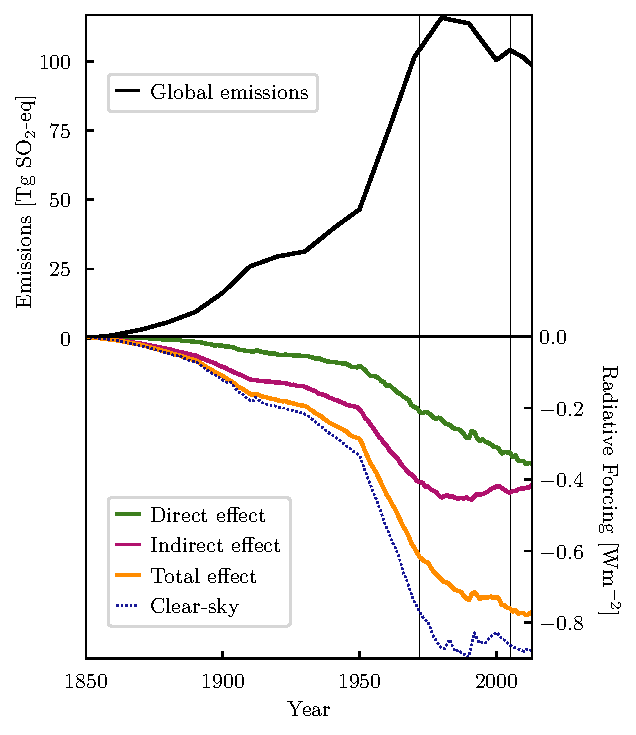
\includegraphics[width=0.5\textwidth]{../../figures/figure1}
            \caption{Historical forcing from anthropogenic aerosols. On the top part is shown the historical global emissions of aerosols and on the bottom part is shown the induced radiative forcing in MPI-ESM1.2-CR. Values are global yearly means. Vertical lines indicate the years 1972 and 2005 when emission levels were similar but led to different total aerosol forcing.}
            \label{fig:figure1}
      \end{figure}

      \subsection{Forcing from Regional Aerosol Sources}
            As detailed in Section \ref{sec:method}, MACv2-SP provided a parametrisation for anthropogenic aerosols, incorporating nine distinct simple-plumes that represent various anthropogenic emission regions. To assess the aerosol forcing from each of these regions, we substituted one plume at a time into the PRP calculation. Fig. \ref{fig:figure2} illustrates the resulting forcing values from each region plotted against their respective aerosol emissions in Tg of SO$_2$ equivalent. Regressing the induced forcing against the associated emission level, we obtain a value of the region aerosol efficiency in Wm$^{-2}$ per Tg of SO$_2$ equivalent.
            In Fig. \ref{fig:figure2}.a., we observe a significant variability in efficiency of the direct effect among major industrial regions, such as Europe, North America, East and South Asia, and Australia. Notably, South Asia exhibits an efficiency 20.10 times greater than Europe, representing the most substantial difference in efficiency across these regions. On the other hand, Fig. \ref{fig:figure2}.b. shows a relatively more consistent relationship between forcing and emissions for the indirect effect across regions. 
            The variation in regional aerosol efficiency explains the persistent increase in the global direct effect. Regions with higher efficiencies have a more substantial impact on the global direct effect while emitting fewer aerosols. This effect becomes particularly evident when considering the shift in aerosol patterns from 1980 to 2005. During this period, aerosol emissions shifted from Europe and North America to Southeast Asia, where higher efficiencies prevailed. Consequently, despite reduced global emissions during this period, the global aerosol forcing continued to rise.
            Subsequent sections delve into the mechanisms that underlie these regional variations in efficiency.

      \begin{figure}
            \centering
            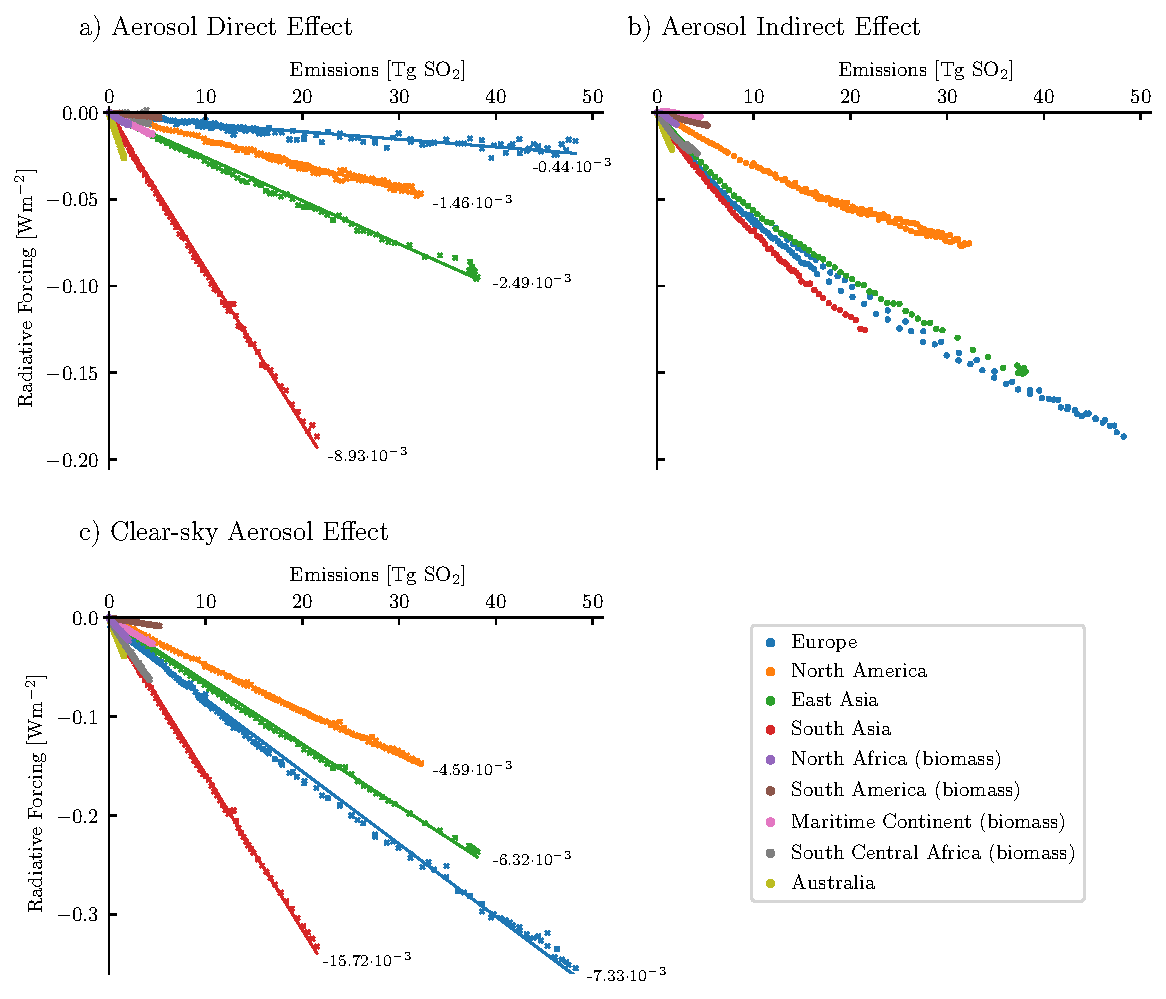
\includegraphics[width=\textwidth]{../../figures/figure2}
            \caption{Aerosol forcing from individual emission regions against regional emission levels. Plots are global yearly means with a) is the direct effect, b) is the indirect effect and c) the clear-sky aerosol effect. Values on the plots are the efficiencies in Wm$^{-2}$ per Tg of SO$_2$ equivalent for the major emission regions, based on linear regression.}
      \label{fig:figure2}
      \end{figure}

      \subsection{All-sky and Clear-sky Aerosol Forcing}\label{sec:clear-sky}
            We examine the outcomes of the PRP performed under both all-sky and clear-sky conditions. The results under all-sky conditions confirm the findings of \citeA{Huusko_2022}: the direct effect primarily occurs in the vicinity of emission sources (see Fig. \ref{fig:figure3}.c.); in contrast, the indirect effect is more pronounced over remote regions (see Fig. \ref{fig:figure3}.b.) and is larger that the direct effect.
            
            In clear-sky conditions, the global aerosol forcing surpasses the global total forcing (including direct and indirect effects) observed under all-sky conditions (see Fig. \ref{fig:figure1}). It is essential to note that, in clear-sky conditions, only the direct effect applies. Interestingly, the clear-sky aerosol forcing is more than twice as large as the direct effect observed in all-sky conditions. This pattern remain consistent across all emission regions, with clear-sky aerosol forcing consistently exceeding the all-sky direct effect (see Fig \ref{fig:figure2}.a. and c.). 
            Under all-sky conditions, the presence of extensive cloud cover results in positive forcing from the direct effect of aerosols (see Fig. \ref{fig:figure3}.c. and e.). In fact, the presence of clouds moderates the net effect of aerosol scattering while amplifying the net effect of aerosol absorption \cite{Li_2022,Bellouin_2020}. With single-scattering albedo of 0.93 and 0.87 for industrial and biomass burning emissions respectively \cite{Stevens_2017}, absorption prevails in the presence of clouds, resulting in positive direct effect of aerosols. %[We confirmed this finding with a simulation in which we set the SSA to 1 (indicating no absorption, only scattering), resulting in solely negative direct effect (not shown). This confirms the significant role of aerosol absorption and its influence on the overall forcing in the presence of clouds.]
            
            In addition, in regions with persistent cloud systems, the negative forcing arising from the indirect effect through clouds and the positive direct effect tend to balance each other (see Fig. \ref{fig:figure3}.a. and e.).
            This mechanism has significant implications for regional emission efficiency. In particular, it explains why Europe, which exhibits weak efficiency under all-sky (Fig. \ref{fig:figure2}.a.) due to positive direct effect at high latitudes (Fig. \ref{fig:figure3}), demonstrates greater efficiency under clear-sky conditions. Looking at clear-sky conditions significantly narrows the gap in regional efficiencies. 
            In South Asia, the efficiency in clear-sky conditions is only 2.1 times greater than in Europe, which is significantly lower than the 20.1 times difference observed in all-sky direct effect. The most pronounced contrast is seen between South Asia and North America, with South Asia showing a efficiency 3.2 times greater than North America.

            The interaction between cloud cover and the direct effect of anthropogenic aerosols emerges as a main factor influencing regional efficiency. This largely explains the consistent increase in aerosol negative forcing despite reduced emissions. As Southeast Asian regions present less cloud cover at the emission sources compared to Europe, the shift in aerosol patterns results in enhanced global direct effect. The presence of clouds in remote regions, stemming from Southeast Asian emission sources, such as over the Indian and Pacific Oceans, maintains the indirect effect despite the pattern shift. Overall, aerosol efficiency is greater in Southeast Asian regions compared to Europe and North America.
            The resulting increase in aerosol efficiency from the shift in aerosol pattern is critical in the enhanced aerosol forcing observed when comparing the mid-1970s to the mid-2000s, even though emissions levels were similar.
            However, the disparity in emission efficiencies among regions remains substantial under clear-sky conditions. The following sections investigate the factors contributing to these regional differences.
            
      \begin{figure}
            \centering
            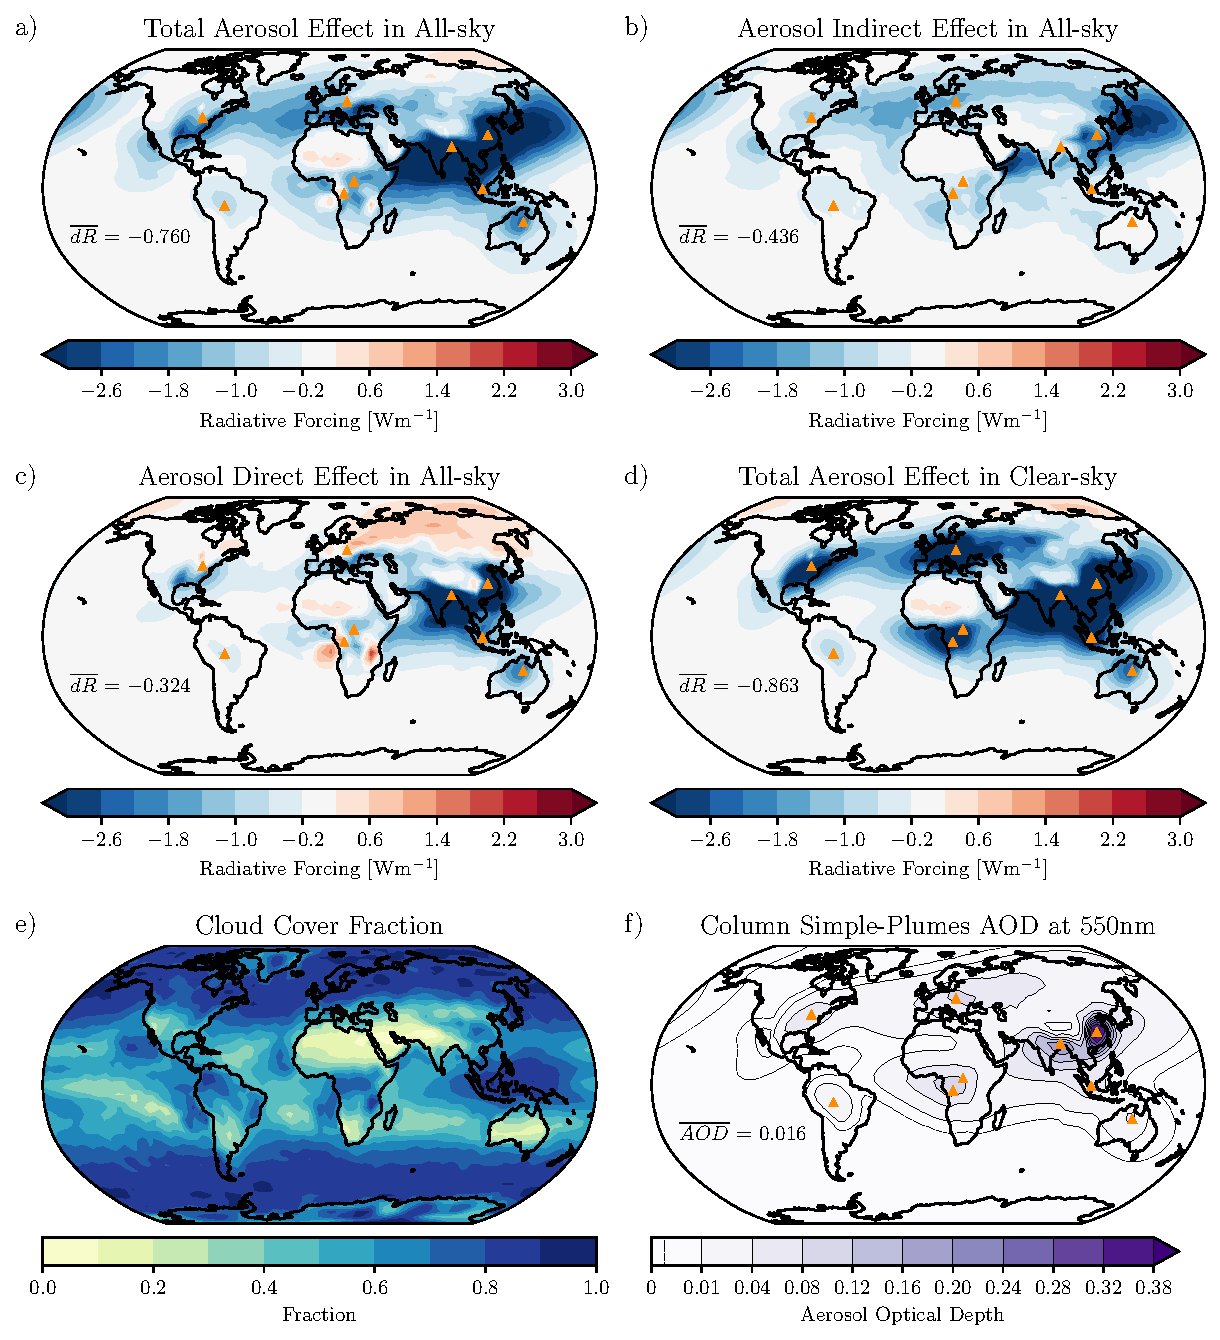
\includegraphics[width=0.9\textwidth]{../../figures/figure3}
            \caption{Present-day (2005) aerosol forcing spatial pattern (yearly mean). Shown is a) the total aerosol forcing, separated into b) the indirect effect and c) the direct effect. d) is the clear-sky aerosol effect and e) is the cloud cover fraction. f) the Column Aerosol Optical Depth at 550nm from the MACv2-SP (Simple-Plumes) parametrisation, with dashed-line showing low AOD value contour (0.0025). Values on the maps are global means.}
            \label{fig:figure3}
      \end{figure}

      \subsection{MACv2-SP Aerosol Representation and Regional Variation}
            The MACv2-SP has been designed to simplify the representation of anthropogenic aerosols in climate models through a straightforward parametrisation. 
            It provides monthly mean Aerosol Optical Depth (AOD) from the ground-based measured 2005 distribution that have been scaled with estimates of historical emissions \cite{Stevens_2017}. 
            Consequently, the AOD in MACv2-SP may not always exhibit a direct proportionality to emissions from various regions due to regional variation in aerosol removal processes. Indeed, wet deposition is the dominant sink of SO$_{\textrm{x}}$ from industrial sources \cite{Textor_2006}, and this deposition particularly prominent over the Eastern costs of North America and East Asia \cite{Rodhe_2002}.

            Fig. \ref{fig:figure4}.a. shows the clear-sky aerosol forcing plotted against the corresponding AOD levels for each region. This representation noticeably reduces the difference in aerosol efficiency between regions. For instance, the efficiency of South Asia is 1.3 greater than that of Europe when measured in Wm$^{-2}$ per unit of optical depth, whereas it was 2.1 greater when measured in Wm$^{-2}$ per unit of emissions (in Tg of SO$_2$-eq).
            Interestingly, when considering AOD levels, both Asian regions exhibit similar efficiencies, which is not the case when considering emissions. 
            Important wet deposition in East Asia contributions to the removal of aerosols \cite{Rodhe_2002}, resulting in lower forcing per unit of emissions in this region. Conversely, South Asia exhibits weaker wet deposition \cite{Rodhe_2002}, allowing for greater forcing per unit of emissions in this region.

            This difference in aerosol removal patterns is the second most important explanation for the continued increase in aerosol forcing despite reduced emissions. The shift in aerosol patterns from Europe and North America towards Southeast Asian regions, with weaker wet deposition, prolongs the residence time of aerosols in the atmosphere, consequently enhancing the aerosol efficiency.
            The last section, we suggest additional explanations for the remaining minor differences in aerosol efficiency between regions.

      \begin{figure}
            \centering
            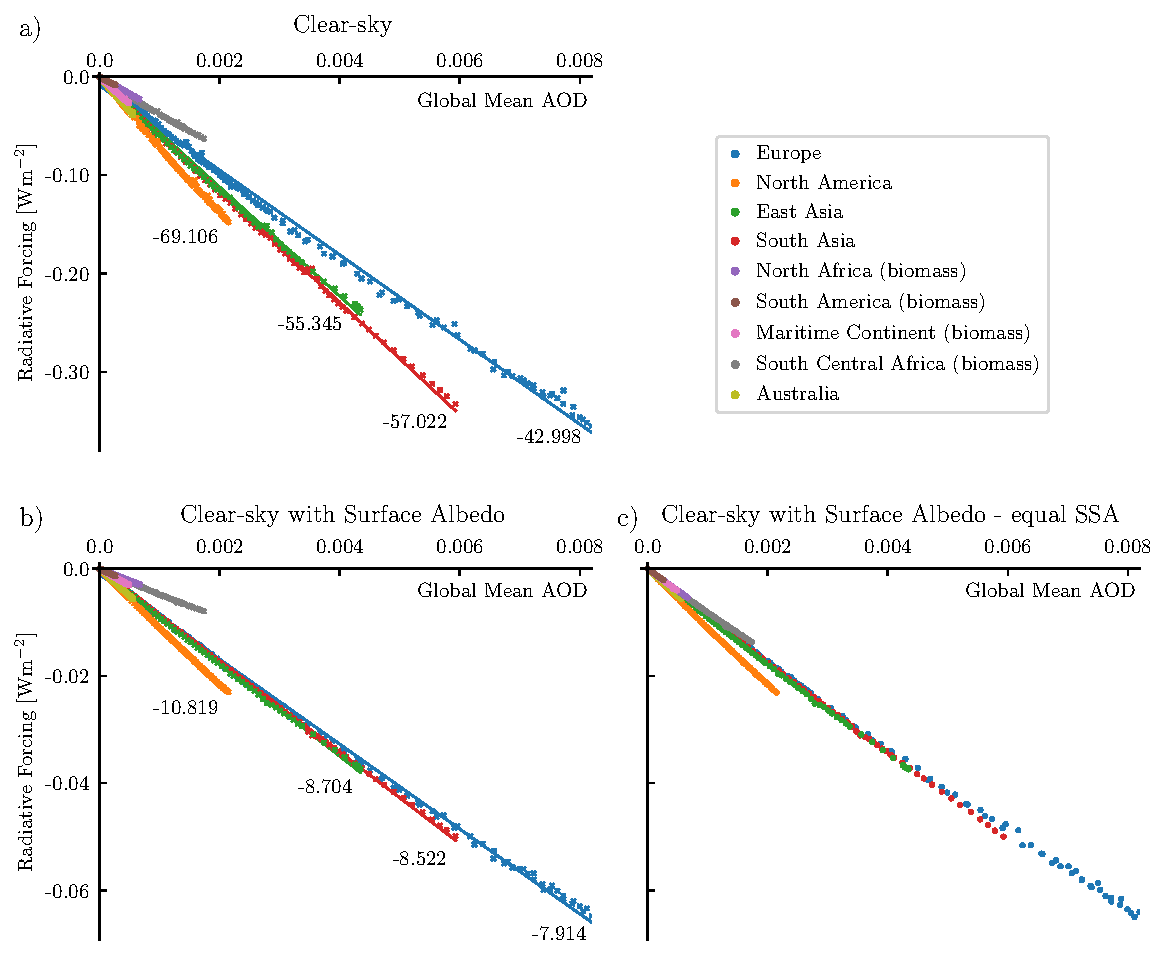
\includegraphics[width=0.9\textwidth]{../../figures/figure4}
            \caption{Aerosol forcing from individual emissions regions against regional column aerosol optical depth. Plots are global yearly means with a) showing the clear-sky aerosol effect, b) the clear-sky aerosol effect adjusted by the surface albedo and c) similar to b) but the Single-Scattering Albedo (SSA) was set to the same value for both industrial and biomass burning sources. Values on the plots are the efficiencies in Wm$^{-2}$ per unit of optical depth of the major emission regions, based on linear regression.}
            \label{fig:figure4}
      \end{figure}

      \subsection{Surface and Aerosol Single-Scattering Albedo}

            The remaining differences in clear-sky efficiency among industrial regions appear to be closely related to surface albedo (Fig. \ref{fig:figure4}.b.). When multiplied by surface albedo, South Asia efficiency in Wm$^{-2}$ per unit of AOD is only 1.08 greater than Europe (against 1.3 without surface albedo adjustments). Similar to cloud cover in Section \ref{sec:clear-sky}, anthropogenic aerosol forcing also depends on the nature of the underlying surface \cite{Li_2022}. In areas with inherently reflective surfaces, aerosol emissions can contribute to the net absorption of shortwave radiation. This clarifies why Europe, which emits aerosols in high-latitudes over snow-covered and icy regions, exhibits weaker efficiency compared to regions with darker surfaces, such as Asia. It's important to note that this effect is primarily observed in clear-sky forcing, as in all-sky conditions, the direct effect is largely influenced by interactions with cloud albedo detailed in Section \ref{sec:clear-sky}. Nonetheless, these findings suggest that a shift in aerosol patterns towards regions with darker surfaces can lead to greater aerosol forcing for similar emission levels.
            
            The distinction between industrial and biomass aerosol emissions affects primarily the Single-Scattering Albedo (SSA) parameter provided by MACv2-SP, which is 0.93 for industrial and 0.87 for biomass burning \cite{Stevens_2017}. The greater shortwave absorption by biomass burning aerosols results in weaker efficiencies when compared to industrial regions. In Fig. \ref{fig:figure4}.c., we provide an identical representation to Fig. \ref{fig:figure4}.b., but with the SSA of biomass regions set to the same value as for industrial regions, effectively eliminating the disparities.
            It's important to note that this observation holds true in all-sky conditions as well, as SSA defines the ratio of scattering efficiency to total extinction efficiency. However, it plays a relatively minor role in the overall discrepancy, given that biomass burning regions have relatively smaller emissions and forcing compared to industrial sources.

\section{Conclusions}
      Our findings indicate a noteworthy increase in aerosol instantaneous radiative forcing, despite a global reduction in aerosol emissions in recent decades. This trend is driven primarily by the direct effect, while the indirect remains more consistent with emission levels. The continuous increase in the direct effect is associated with significant regional shifts in emissions. Historically, aerosols were predominantly emitted from Europe and North America in the 1970s, but today, their primary sources have shifted to Southeast Asian regions. 
      
      The primary factor driving this disparity is the influence of cloud cover. High-latitude regions, characterised by substantial cloud cover, tend to enhance aerosol absorption, resulting in a positive direct effect. In contrast, the recent shift of aerosol emissions to Southeast Asia, where cloud cover is generally reduced at the source, has led to a more negative aerosol direct effect.
      The second significant contributor to this discrepancy is the regional variation in aerosol lifetime within the atmosphere. Comparatively stable atmospheric conditions in South Asia with weaker wet aerosol deposition, as opposed to North America, have led to a greater efficiency in terms of radiative forcing per unit of emissions with the shift of emissions to South Asia. 

      Moreover, high-latitude regions are distinguished by their reflective surfaces, which tend to mitigate the aerosol direct effect, in contrast to the absorbing surfaces prevalent in Asia. However, surface albedo plays a relatively minor role, as the reflective surfaces in Northern Europe are often covered by clouds.
      Finally, the nature of aerosol particles can also influence the efficiency per unit of emissions. In recent decades, emerging biomass burning sources in Southern countries have been emitting a greater quantity of absorbing aerosols, which acts to dampen the direct effect efficiency. Nevertheless, since these biomass burning emissions remain relatively small in comparison to industrial sources, this has not offset the global negative increase in the direct effect.

      When comparing to other global climate models, MPI-ESM1.2 falls into the low range of aerosol forcing \cite{Fiedler_2023}. The range of forcing is due to indirect effect. From our results, we suggest that models with weaker indirect effect relative to direct effect could present more inconsistent forcing with emissions, while the aerosol forcing from models with strong indirect effect will be more consistent with emissions. 
      The processes we described can help explain a variety of aerosol forcing evolution in CMIP6
      
%  Numbered lines in equations:
%  To add line numbers to lines in equations,
%  \begin{linenomath*}
%  \begin{equation}
%  \end{equation}
%  \end{linenomath*}



%% Enter Figures and Tables near as possible to where they are first mentioned:
%
% DO NOT USE \psfrag or \subfigure commands.
%
% Figure captions go below the figure.
% Acronyms used in figure captions will be spelled out in the final, published version.

% Table titles go above tables;  other caption information
%  should be placed in last line of the table, using
% \multicolumn2l{$^a$ This is a table note.}
% NOTE that there is no difference between table caption and table heading in the final, published version
%
%----------------
% EXAMPLE FIGURES
%
% \begin{figure}
% \includegraphics{example.png}
% \caption{caption}
% \end{figure}
%
% Giving latex a width will help it to scale the figure properly. A simple trick is to use \textwidth. Try this if large figures run off the side of the page.
% \begin{figure}
% \noindent\includegraphics[width=\textwidth]{anothersample.png}
%\caption{caption}
%\label{pngfiguresample}
%\end{figure}
%
%
% If you get an error about an unknown bounding box, try specifying the width and height of the figure with the natwidth and natheight options. This is common when trying to add a PDF figure without pdflatex.
% \begin{figure}
% \noindent\includegraphics[natwidth=800px,natheight=600px]{samplefigure.pdf}
%\caption{caption}
%\label{pdffiguresample}
%\end{figure}
%
%
% PDFLatex does not seem to be able to process EPS figures. You may want to try the epstopdf package.
%

%
% ---------------
% EXAMPLE TABLE
%
% \begin{table}
% \caption{Time of the Transition Between Phase 1 and Phase 2$^{a}$}
% \centering
% \begin{tabular}{l c}
% \hline
%  Run  & Time (min)  \\
% \hline
%   $l1$  & 260   \\
%   $l2$  & 300   \\
%   $l3$  & 340   \\
%   $h1$  & 270   \\
%   $h2$  & 250   \\
%   $h3$  & 380   \\
%   $r1$  & 370   \\
%   $r2$  & 390   \\
% \hline
% \multicolumn{2}{l}{$^{a}$Footnote text here.}
% \end{tabular}
% \end{table}

%%%%%%%%%%%%%%%%%%%%%%%%%%%%%%%%%%%%%%%%%%%%%%%
% SIDEWAYS FIGURES and TABLES
% AGU prefers the use of {sidewaystable} over {landscapetable} as it causes fewer problems.
%
% \begin{sidewaysfigure}
% \includegraphics[width=20pc]{figsamp}
% \caption{caption here}
% \label{newfig}
% \end{sidewaysfigure}
%
%  \begin{sidewaystable}
%  \caption{Caption here}
% \label{tab:signif_gap_clos}
%  \begin{tabular}{ccc}
% one&two&three\\
% four&five&six
%  \end{tabular}
%  \end{sidewaystable}

%% If using numbered lines, please surround equations with \begin{linenomath*}...\end{linenomath*}
%\begin{linenomath*}
%\begin{equation}
%y|{f} \sim g(m, \sigma),
%\end{equation}
%\end{linenomath*}

%%% End of body of article

%%%%%%%%%%%%%%%%%%%%%%%%%%%%%%%%%%%%%%%%%%%%%%%
%% Optional Appendices go here
%
% The \appendix command resets counters and redefines section heads
%
% After typing \appendix
%
%\section{Here Is Appendix Title}
% will show
% A: Here Is Appendix Title
%
%\appendix
%\section{Here is a sample appendix}

%%%%%%%%%%%%%%%%%%%%%%%%%%%%%%%%%%%%%%%%%%%%%%%
% Optional Glossary, Notation or Acronym section goes here:
%
% Glossary is only allowed in Reviews of Geophysics
%  \begin{glossary}
%  \term{Term}
%   Term Definition here
%  \term{Term}
%   Term Definition here
%  \term{Term}
%   Term Definition here
%  \end{glossary}


%%%%%%%%%%%%%%%%%%%%%%%%%%%%%%%%%%%%%%%%%%%%%%%
% Acronyms
%% NOTE that acronyms in the final published version will be spelled out when used in figure captions.
%   \begin{acronyms}
%   \acro{Acronym}
%   Definition here
%   \acro{EMOS}
%   Ensemble model output statistics
%   \acro{ECMWF}
%   Centre for Medium-Range Weather Forecasts
%   \end{acronyms}


%%%%%%%%%%%%%%%%%%%%%%%%%%%%%%%%%%%%%%%%%%%%%%%
% Notation
%   \begin{notation}
%   \notation{$a+b$} Notation Definition here
%   \notation{$e=mc^2$}
%   Equation in German-born physicist Albert Einstein's theory of special
%  relativity that showed that the increased relativistic mass ($m$) of a
%  body comes from the energy of motion of the body—that is, its kinetic
%  energy ($E$)—divided by the speed of light squared ($c^2$).
%   \end{notation}




%%%%%%%%%%%%%%%%%%%%%%%%%%%%%%%%%%%%%%%%%%%%%%%
%
% DATA SECTION and ACKNOWLEDGMENTS
%
%%%%%%%%%%%%%%%%%%%%%%%%%%%%%%%%%%%%%%%%%%%%%%%

\section*{Open Research Section}
The source code for MPI-ESM1.2 can be accessed via https://mpimet.mpg.de/en/science/models/mpi-esm \cite{Mauritsen_2019}. Additionally, the specific parts of the code that were modified or implemented for this study, as well as the output data and Python scripts used in producing the figures presented in this paper, are accessible through Zenodo at [link] \cite{}


% This section MUST contain a statement that describes where the data supporting the conclusions can be obtained. Data cannot be listed as ''Available from authors'' or stored solely in supporting information. Citations to archived data should be included in your reference list. Wiley will publish it as a separate section on the paper’s page. Examples and complete information are here:
%https://www.agu.org/Publish with AGU/Publish/Author Resources/Data for Authors


\acknowledgments
The computations resources were provided by the National Academic Infrastructure for Supercomputing in Sweden (NAISS) and the Swedish National Infrastructure for Computing (SNIC) partially funded by the Swedish Research Council through grant agreements no. 2022-06725.
%Enter acknowledgments here. This section is to acknowledge funding, thank colleagues, enter any secondary affiliations, and so on.


%%%%%%%%%%%%%%%%%%%%%%%%%%%%%%%%%%%%%%%%%%%%%%%
% REFERENCES and BIBLIOGRAPHY
%
\bibliography{/home/anthe/misu/paper_aerosols/latex/bibtex/paper_aerosols.bib} 
 %don't specify the file extension
% don't specify bibliographystyle
%
%%%%%%%%%%%%%%%%%%%%%%%%%%%%%%%%%%%%%%%%%%%%%%%

%\bibliography{ enter your bibtex bibliography filename here }



%Reference citation instructions and examples:
%
% Please use ONLY \cite and \citeA for reference citations.
% \cite for parenthetical references
% ...as shown in recent studies (Simpson et al., 2019)
% \citeA for in-text citations
% ...Simpson et al. (2019) have shown...
%
%
%...as shown by \citeA{jskilby}.
%...as shown by \citeA{lewin76}, \citeA{carson86}, \citeA{bartoldy02}, and \citeA{rinaldi03}.
%...has been shown \cite{jskilbye}.
%...has been shown \cite{lewin76,carson86,bartoldy02,rinaldi03}.
%... \cite <i.e.>[]{lewin76,carson86,bartoldy02,rinaldi03}.
%...has been shown by \cite <e.g.,>[and others]{lewin76}.
%
% apacite uses < > for prenotes and [ ] for postnotes
% DO NOT use other cite commands (e.g., \citet, \citep, \citeyear, \nocite, \citealp, etc.).
%



\end{document}



More Information and Advice:

%%%%%%%%%%%%%%%%%%%%%%%%%%%%%%%%%%%%%%%%%%%%%%%
%
%  SECTION HEADS
%
%%%%%%%%%%%%%%%%%%%%%%%%%%%%%%%%%%%%%%%%%%%%%%%

% Capitalize the first letter of each word (except for
% prepositions, conjunctions, and articles that are
% three or fewer letters).

% AGU follows standard outline style; therefore, there cannot be a section 1 without
% a section 2, or a section 2.3.1 without a section 2.3.2.
% Please make sure your section numbers are balanced.
% ---------------
% Level 1 head
%
% Use the \section{} command to identify level 1 heads;
% type the appropriate head wording between the curly
% brackets, as shown below.
%
%An example:
%\section{Level 1 Head: Introduction}
%
% ---------------
% Level 2 head
%
% Use the \subsection{} command to identify level 2 heads.
%An example:
%\subsection{Level 2 Head}
%
% ---------------
% Level 3 head
%
% Use the \subsubsection{} command to identify level 3 heads
%An example:
%\subsubsection{Level 3 Head}
%
%---------------
% Level 4 head
%
% Use the \subsubsubsection{} command to identify level 3 heads
% An example:
%\subsubsubsection{Level 4 Head} An example.
%
%%%%%%%%%%%%%%%%%%%%%%%%%%%%%%%%%%%%%%%%%%%%%%%
%
%  IN-TEXT LISTS
%
%%%%%%%%%%%%%%%%%%%%%%%%%%%%%%%%%%%%%%%%%%%%%%%
%
% Do not use bulleted lists; enumerated lists are okay.
% \begin{enumerate}
% \item
% \item
% \item
% \end{enumerate}
%
%%%%%%%%%%%%%%%%%%%%%%%%%%%%%%%%%%%%%%%%%%%%%%%
%
%  EQUATIONS
%
%%%%%%%%%%%%%%%%%%%%%%%%%%%%%%%%%%%%%%%%%%%%%%%

% Single-line equations are centered.
% Equation arrays will appear left-aligned.

Math coded inside display math mode \[ ...\]
 will not be numbered, e.g.,:
 \[ x^2=y^2 + z^2\]

 Math coded inside \begin{equation} and \end{equation} will
 be automatically numbered, e.g.,:
 \begin{equation}
 x^2=y^2 + z^2
 \end{equation}


% To create multiline equations, use the
% \begin{eqnarray} and \end{eqnarray} environment
% as demonstrated below.
\begin{eqnarray}
  x_{1} & = & (x - x_{0}) \cos \Theta \nonumber \\
        && + (y - y_{0}) \sin \Theta  \nonumber \\
  y_{1} & = & -(x - x_{0}) \sin \Theta \nonumber \\
        && + (y - y_{0}) \cos \Theta.
\end{eqnarray}

%If you don't want an equation number, use the star form:
%\begin{eqnarray*}...\end{eqnarray*}

% Break each line at a sign of operation
% (+, -, etc.) if possible, with the sign of operation
% on the new line.

% Indent second and subsequent lines to align with
% the first character following the equal sign on the
% first line.

% Use an \hspace{} command to insert horizontal space
% into your equation if necessary. Place an appropriate
% unit of measure between the curly braces, e.g.
% \hspace{1in}; you may have to experiment to achieve
% the correct amount of space.


%%%%%%%%%%%%%%%%%%%%%%%%%%%%%%%%%%%%%%%%%%%%%%%
%
%  EQUATION NUMBERING: COUNTER
%
%%%%%%%%%%%%%%%%%%%%%%%%%%%%%%%%%%%%%%%%%%%%%%%

% You may change equation numbering by resetting
% the equation counter or by explicitly numbering
% an equation.

% To explicitly number an equation, type \eqnum{}
% (with the desired number between the brackets)
% after the \begin{equation} or \begin{eqnarray}
% command.  The \eqnum{} command will affect only
% the equation it appears with; LaTeX will number
% any equations appearing later in the manuscript
% according to the equation counter.
%

% If you have a multiline equation that needs only
% one equation number, use a \nonumber command in
% front of the double backslashes (\\) as shown in
% the multiline equation above.

% If you are using line numbers, remember to surround
% equations with \begin{linenomath*}...\end{linenomath*}

%  To add line numbers to lines in equations:
%  \begin{linenomath*}
%  \begin{equation}
%  \end{equation}
%  \end{linenomath*}



